\documentclass[10pt,a4paper]{article}
\usepackage[utf8]{inputenc}
\usepackage[spanish]{babel}
\usepackage{geometry,booktabs,graphicx,float,hyperref}
\graphicspath{{../04_graficos/}{{04_graficos/}}{{graficos/}}{{./}}}
\geometry{margin=1.55cm}
\setlength{\parskip}{2pt}
\setlength{\parindent}{0pt}
\title{\vspace{-1.2cm}\textbf{Informe ejecutivo Taller 1: La Beta de los Pobres}}
\author{Julián Duarte -- Valoración de Activos (DEFI 2)}
\date{Agosto de 2026}
\begin{document}
\maketitle
\textbf{Pregunta.} ¿Qué revela el CAPM sobre SOL frente al NCI y sobre nueve acciones de bajo precio frente a sus ETF sectoriales? La evidencia muestra que el 25\% anual sin caídas no es defendible: los retornos altos observados vienen acompañados de drawdowns, CVaR e iliquidez severa.

\textbf{Datos.} Ventana común: agosto de 2024 a agosto de 2026. SOL se compara con NCI; Tecnología con XLK; Biotecnología con XBI; Energía con XLE. Se usan precios ajustados y volumen de Yahoo Finance, NCI suministrado por el profesor y DGS3MO de FRED. La tasa diaria usa ACT/365 para cripto y 252 días para acciones. Los tickers son KOPN, MVIS, LIDR, GERN, CTMX, OCGN, BORR, KLXE y TTI; TTI se documenta como acción de bajo precio bajo la excepción menor a USD 10.

\begin{table}[H]\centering\scriptsize
\caption{CAPM con errores HAC Newey--West}
\begin{tabular}{lccccccc}\toprule
Activo & Bench. & $\alpha$ anual & $\beta$ & IC 95\% $\beta$ & $R^2$ & Ret. obs. & Ret. CAPM\\\midrule
SOL & NCI & -28.86\% & 1.25 & [1.16,1.34] & 0.66 & 4.62\% & 33.48\% \\
KOPN & XLK & 80.66\% & 1.82 & [1.57,2.07] & 0.23 & 129.96\% & 49.31\% \\
MVIS & XLK & -82.91\% & 1.16 & [0.84,1.47] & 0.09 & -50.14\% & 32.76\% \\
LIDR & XLK & 60.13\% & 1.27 & [0.96,1.58] & 0.04 & 95.74\% & 35.61\% \\
GERN & XBI & -64.14\% & 1.12 & [0.98,1.27] & 0.22 & -32.87\% & 31.27\% \\
CTMX & XBI & 72.75\% & 1.52 & [0.90,2.13] & 0.11 & 113.54\% & 40.79\% \\
OCGN & XBI & -2.30\% & 1.15 & [0.96,1.34] & 0.17 & 29.60\% & 31.90\% \\
BORR & XLE & -29.54\% & 1.36 & [1.11,1.60] & 0.27 & -0.62\% & 28.91\% \\
KLXE & XLE & -67.77\% & 1.94 & [1.59,2.29] & 0.20 & -28.20\% & 39.56\% \\
TTI & XLE & 29.83\% & 1.14 & [0.87,1.40] & 0.18 & 54.68\% & 24.85\% \\
\bottomrule\end{tabular}\end{table}

\begin{table}[H]\centering\scriptsize
\caption{Riesgo, desempeño y liquidez}
\begin{tabular}{lccccccc}\toprule
Activo & Vol. & Sharpe & MDD & CVaR 95\% & $r=0$ & $\beta^-$ & Amihud\\\midrule
SOL & 88.00\% & 0.01 & -75.45\% & -9.99\% & 0.0\% & 1.24 & 6.19e-14 \\
KOPN & 103.28\% & 1.22 & -63.55\% & -12.35\% & 3.6\% & 2.21 & 1.46e-08 \\
MVIS & 104.55\% & -0.52 & -93.92\% & -15.14\% & 11.0\% & 1.12 & 1.08e-08 \\
LIDR & 165.91\% & 0.55 & -82.98\% & -14.09\% & 3.8\% & 1.31 & 9.54e-08 \\
GERN & 66.55\% & -0.55 & -77.47\% & -8.69\% & 8.0\% & 1.18 & 1.81e-09 \\
CTMX & 128.34\% & 0.85 & -67.02\% & -11.49\% & 3.2\% & 1.26 & 1.97e-08 \\
OCGN & 77.83\% & 0.33 & -61.20\% & -9.18\% & 5.8\% & 1.41 & 7.90e-09 \\
BORR & 61.72\% & -0.08 & -74.78\% & -8.00\% & 4.4\% & 1.30 & 1.95e-09 \\
KLXE & 100.92\% & -0.32 & -79.89\% & -12.95\% & 3.4\% & 2.10 & 1.06e-07 \\
TTI & 62.21\% & 0.81 & -57.23\% & -8.40\% & 2.0\% & 1.30 & 4.33e-09 \\
\bottomrule\end{tabular}\end{table}

\begin{figure}[H]\centering
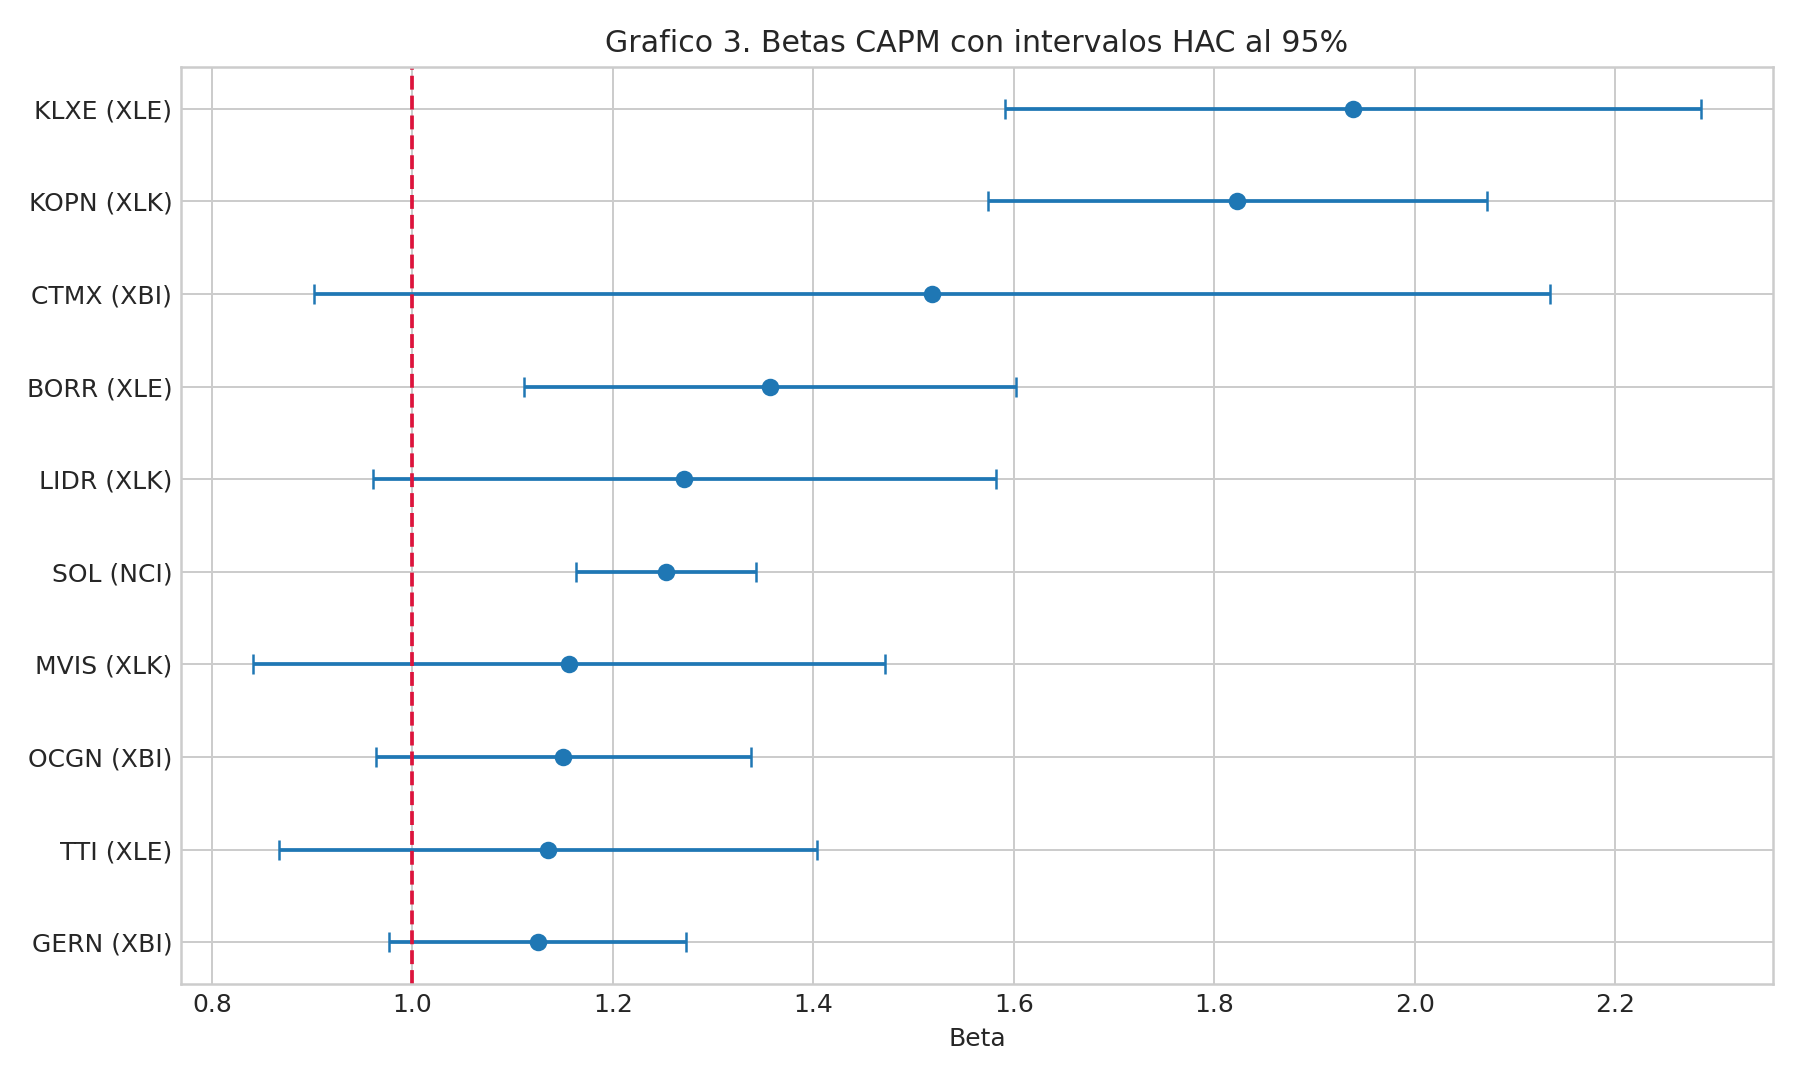
\includegraphics[width=.92\linewidth]{grafico_3_forest_plot_betas.png}
\caption{Las betas se interpretan frente a su benchmark propio; una beta alta en XLE no equivale directamente a una beta alta en NCI.}
\end{figure}

\textbf{Hallazgos.} SOL tiene una exposición sistemática material frente al mercado cripto y conserva riesgo bajista. En acciones de bajo precio, la beta debe leerse junto con liquidez: retornos cero, bajo volumen monetario y cambios fuertes entre beta contemporánea, Dimson y winsorizada sugieren posible negociación no sincrónica. Las acciones de energía y tecnología concentran episodios de drawdown severo; biotecnología mantiene sensibilidad alta a choques sectoriales y regulatorios.

\textbf{Hipótesis.} Se contrasta $H_0:\beta=1$ con el estadístico $(\hat\beta-1)/SE(\hat\beta)$ y $H_0:\alpha=0$ con p-valores HAC. La decisión no se basa solo en significancia: se reportan intervalos, tamaño del efecto y significado financiero.

\textbf{Recomendación.} Para conservación, liquidar posiciones con iliquidez extrema o drawdowns incompatibles con el mandato y priorizar T-Bills/ETF diversificados. Para crecimiento, SOL solo puede mantenerse como exposición acotada al mercado cripto, no como fuente de retorno garantizado. Para especulación acotada, limitar cada acción de bajo precio a 1\%-2\% del portafolio y presupuestar pérdida máxima; ninguna posición justifica prometer 25\% anual sin caídas.

\textbf{Limitaciones.} El CAPM es lineal, usa betas históricas y no captura eventos discretos como splits, aprobaciones regulatorias, riesgo de financiación o shocks de liquidez. Por eso la recomendación combina beta, drawdown, CVaR, beta bajista, Amihud y estabilidad temporal.
\end{document}
